\documentclass[11pt]{article}
\usepackage[a4paper,margin=1in]{geometry}
\reversemarginpar
\usepackage{mathtools, amsthm, amssymb, amsmath}
\usepackage{multicol}
\usepackage{todonotes}

\usepackage{subcaption}
\usepackage{longtable}

\usepackage[style=numeric, sorting=none]{biblatex}
\addbibresource{MV.bib}
\usepackage{hyperref}

\usepackage{graphicx}
\graphicspath{{./picture/}}

\usepackage{subcaption}

\usepackage{tikz}
\usetikzlibrary{positioning}

\usepackage{rotating}

\newtheorem{theorem}{Theorem}[section]
\theoremstyle{definition}
\newtheorem{definition}[theorem]{Definition}
\newtheorem{example}[theorem]{Example}

\DeclareMathOperator{\dom}{dom}

\title{Generating of Music Variations: Dynamical Systems Approach}
\author{Rajamangala University of Technology Thanyaburi\\Kanatsanun Sub-udom\\Wannasa Rianthong\\Patipan Somwong}

\begin{document}
\maketitle
\begin{abstract}
This paper introduces a new method for diversifying musical compositions to address the issue of composer burnout. By utilizing the characteristics of chaotic dynamical systems, well-known for their sensitivity to initial conditions, this approach combines melodic variation with an extended rhythmic structure. The proposed technique entails the mapping of musical data onto a chaotic attractor, which generates a new variation as the system's trajectories evolve. This expansion of rhythm is achieved by prolonging the duration of musical notes, resulting in a natural blending of melodic and rhythmic elements. The objective is to offer composers a systematic and creative tool for exploring innovative musical concepts, relieving creative fatigue, and invigorating the compositional process.
\end{abstract}

\section{Introduction}
Music variation serves as a catalyst for creative thinking in the songwriting process. It offers flexibility, capable of generating patterns ranging from close replicas to entirely different ones. The outcome depends on the composer's desires. When applied to compositions, it's like creating another version of the same song, making the music open to change every time it's heard. In the past, composers often employed techniques like inversion, retrograde or sections of music to expand upon the original musical content. However, these techniques gradually lost their appeal and were seen as tiresome. Music variation steps in to fill this gap. This technique opens up possibilities for composers to create entirely new musical patterns without being tied to the original framework. The written notes can transform with every listen, resulting in dynamic and fresh music akin to a rocket launching pad propelling composers into an unrestricted musical universe.

Nowadays, artificial intelligence (AI) technologies have significantly advanced, enabling them to create music with ever-increasing proficiency \cite{bonnici_music_2021}. 
Well-known AI music generation platforms such as  Mubert \cite{mubert_website} and 
Musicity \cite{musicfy_website} empower users with real-time music generation capabilities, 
enabling them to effortlessly select their preferred genre or mood and promptly receive a personalized soundtrack tailored to their preferences. On the other hand, Soundraw \cite{soundraw_website} and Boomy \cite{boomy_website} function as AI-driven music creation tools, furnishing a diverse array of features to aid users in sculpting their musical opuses with ease. Meanwhile, AIVA \cite{aiva_website} harnesses the power of deep learning to craft original music closely resembling the distinctive style of a particular artist or genre. Users can furnish reference tracks or articulate their desired musical aesthetics, prompting AIVA to generate fresh compositions that align precisely with their specifications. However, these technologies often require high computational resources, making them unable to run on devices with low processing power. Additionally, some AI music composition tools may produce music in limited styles.

If the limitations of AI music composition technology remain unaddressed, it will have repercussions. Firstly, aspiring artists and musicians will miss out on the opportunity to use these tools due to limited access, as most people lack high-performance equipment. Furthermore, all music generated by AI may start to sound similar, potentially leading to a lack of musical diversity.The paper thus aims to address the aforementioned issue by employing a multi-step process. Initially, it utilizes melodic variation with expanded rhythm, which is then translated into numerical values. These numerical values are then input into a chaotic dynamical system, resulting in a new set of numbers different from the original. Finally, these numbers are mapped back to musical notes, resulting in the creation of a new piece of music. This method requires fewer computing resources compared to using AI music composition technology and allows for the creation of diverse musical compositions depending on the original song, initial values, and equations used.

In this work, We explore the theory behind chaotic system equations and the basic music theory in Section \ref{sec: literaturereview}. In Section \ref{sec: mainresult}, we will commence by explaining the theory and examples from \cite{dabby_musical_1996}. Following that, we will utilize melodic variation with expanded rhythm in Subsection \ref{subsec: melodicvariationwithexpandedrhythm} to illustrate our subsequent workflow. In Section \ref{sec: discussion}, we will present and exchange ideas, opinions, and relevant information. Finally,  we summarize the solutions and insights we have derived to address the issues discussed in this paper succinctly and conclusively, in Section \ref{sec: conclusion}

\section{Literature Review}
\label{sec: literaturereview}

\begin{figure}
\centering
\begin{subfigure}{0.45\textwidth}
  \centering
  \includegraphics[trim=2cm 2cm 2cm 2cm, clip, scale=0.3]{Lorenz1.pdf}
  \caption{The Lorenz system with initial condition $(1,1,1)$.}
  \label{subfig1:mp}
\end{subfigure}\hfill
\begin{subfigure}{0.45\textwidth}
  \centering
  \includegraphics[trim=2cm 2cm 2cm 2cm, clip, scale=0.3]{Lorenz2.pdf}
  \caption{The Lorenz system with initial condition $(0.999,1,1)$.}
  \label{subfig2:mp}
\end{subfigure}
\caption{Chaotic behavior of the Lorenz system with different initial conditions.}
\label{fig:LE}
\end{figure}

In music theory \cite{carter_music_2016}, a musical note is a symbol on sheet music that represents pitch, which refers to the highness or lowness of a sound.  Notes are typically designated by the letters A through G, corresponding to the solfege syllables (Do, Re, Mi, Fa, Sol, La, Ti).  Musical notation also incorporates numbers to specify the octave of a pitch. For instance, C4 represents middle C, while C3 is an octave lower and C5 is an octave higher. A deeper understanding of musical notation systems can be found in resources on music theory.

Musical note duration refers to the length of time a musical note is held, which is a fundamental element in creating rhythm within a piece of music.  Traditionally, note durations are represented using fractions of a whole note. Common note values include the whole note (4 beats), half note (2 beats), quarter note (1 beat), eighth note (0.5 beats), and sixteenth note (0.25 beats).

Given a note duration denoted by $\phi$ and divided into $D$ equal parts, the duration, $R$, of each individual division is defined by the following equation:
$$ R = \frac{\phi}{D}.  $$
\textbf{Note:} In musical theory, equal parts refers to divisions that all have the same duration.

In this paper, let $\mathbb{N}_n$ denote the sequence of natural number with $n$-elements defined by $\mathbb{N}_n = \{ 1, 2, \dots, n \}$ and $\mathbb{R}^n$ be a n-dimensional euclidean space and $\dot{x}(t)$ represents a system of ordinary differential equations. Here,  $\dot{x}$ represents the derivative of $x$ with respect to time.

\section{Main Result}
\label{sec: mainresult}
In this section, we present two methods for generating musical variations. Which is the musical variations from a chaotic mapping method and melodic variation with expanded rhythm method. In the first example, we illustrate how a chaotic mapping can be used to generate variations in musical pitch. In the second example, we combine the musical variations from a chaotic mapping method with melodic variation with Expanded Rhythm Method to create more interesting musical variations.

\subsection{Musical Variations from a Chaotic Mapping}

\label{ss: mvfacm}
For a musical sheet, let $m$ be a positive integer representing a number of notes, $\{p_k\}_{k=0}^{m-1}$ be a sequence of music pitches and   
\begin{equation} \label{eq: odes}
\dot{x}(t) = f(t,x)
\end{equation}
be a chaotic dynamical system with an initial condition $x(0) \in \mathbb{R}^n$, where $x(t) = \left(x_1(t), \ldots, x_n(t)\right)$ is differntiable for all $t \geq 0$.
Let $f: \mathbb{R}_{+} \times \mathbb{R}^n \to \mathbb{R}^n$ is a continuous function. 
Given a sequece
$ \displaystyle\left\{\phi_i(kh) \right\}_{k=0}^{m-1}$ 
for some $i \in \mathbb{N}_n$, where $\phi_i:\mathbb{R}_+ \to \mathbb{R}$ is a numerical solution in $i$-th component to \eqref{eq: odes} with a step size of $h$.
Let $g$ be a mapping defined by 
$g(\phi_i(kh)) := p_k$ for all $k \in \{0\}\cup\mathbb{N}_{m-1}$.

In order to generate a new variation of the sequence $ \left\{\tilde{\phi}_i(kh) \right\}_{k=0}^{m-1} $, where $\tilde{\phi}_i$ is a numerical solution with a new initial condition $\tilde{x}(0) \in \mathbb{R}^n$ $i$-th component to \eqref{eq: odes}, 
when $\tilde{x}(0)$ located not far from $x(0)$, i.e., $ \left\lVert x(0) - \tilde{x}(0) \right\rVert \leq d$ for some small positve number $d \in \mathbb{R}$. Consequence, we define another mapping $l$ by: 
\[ l\left(\tilde{\phi}_i(kh)\right) := 
\begin{cases}
  g(\phi_i(b)) & \text{ if }\exists a, b \in \dom{\phi_i} \text{ s.t. } \phi_i(a) < \tilde{\phi}(kh) \leq \phi_i(b), \\
  & \text{ and } \nexists c \in \dom{\phi_i} \text{ s.t. } \phi_i(a) < \phi_i(c) \leq \phi_i(b), \\
  g(\phi_i(a)) & \text{ if } \tilde{\phi}(kh) < \phi_i(a) \text{ for all } a \in \dom{\phi_i}, \\
  g(\phi_i(b)) & \text{ otherwise},
\end{cases}
\]

which produce a new sequence $\{ l(\tilde{v}_k) \}_{k = 0}^{m - 1}$. 

\begin{example}
Consider the musical sheet of 12 variations on Ah vous dirai-je Maman \cite{hinson_12_1987} in the first 3 bars, illustrated in Figure \ref{fig:Dabby1}. We can convert this musical sheet into a sequence $\{p_k\}_{k=0}^{10}$, where $p_k \in \{C4, C4, G4, G4, A4, A4, G4, F4, F4, E4, E4 \}$ denotes the musical pitch at index $k$. Let 
\begin{equation} \label{eq: re}
\dot{x}(t) = f(t , x_n)
\end{equation} be a Lorenz system with chaotic behavior by giving Lorenz parameters $r = 28, \sigma=10$ and $b = 2.6667$. Then, let the numerical solution of \eqref{eq: re} with initial condition $(1,1,1)$ and a step size of $h=0.01$ be a sequence $\{ \phi_1(kh) \}_{k=0}^{10}$, where $ \phi_1(kh) \in \{1.00, 1.29, 2.13, 3.74, 6.54, 11.04, 16.69, 19.56, 15.37, 7.55, 1.20\}$ denotes the numerical solution at index $k$ and $\phi_1(kh)$ is a numerical solution in first component to \eqref{eq: re}. we can create a mapping $g$ from the real values to musical pitches as follows:
\begin{center}
\begin{tabular}{|c||c|c|c|c|c|c|}
\hline
$ \phi_1(kh) $ & $1.00$ & $1.29$ & $2.13$ & $3.74$ & $6.54$ & $11.04$ \\
\hline
$g(\phi_1(kh))$ & C4 & C4 & G4 & G4 & A4 & A4 \\
\hline
$\phi_1(kh)$ & $16.69$ & $19.56$ & $15.37$ & $7.55$ & $1.20$ & \\
\hline
$g(\phi_1(kh))$ & G4 & F4 & F4 & E4 & E4 &  \\
\hline
\end{tabular}
\end{center}
Consequence, we generate a new trajectory sequence $\left\{\tilde{\phi}_1(kh) \right\}_{k=0}^{10}$ with an initial condition of $(1.01,1,1)$ and a step size of $h=0.01$, where $\tilde{\phi}_1(kh) \in \{ 1.01, 1.30, 2.15, 3.76, 6.58, 11.10, 16.73, 19.55, 15.30, 7.48, 1.15 \}$ denotes the numerical solution at index $k$ and $\tilde{\phi_1}(kh)$ is a numerical solution in first component to \eqref{eq: re}. We can create a mapping $l$ from the real values to new musical pitches as follows:
\begin{center}
\begin{tabular}{|c||c|c|c|c|c|c|}
\hline
$\tilde{\phi}_1(kh)$ & $1.01$ & $1.30$ & $2.15$ & $3.76$ & $6.58$ & $11.10$ \\
\hline
$l(\tilde{\phi}_1(kh))$ & E4 & G4 & G4 & A4 & E4 & F4 \\
\hline
$\tilde{\phi}_1(kh)$ & $16.73$ & $19.55$ & $15.30$ & $7.48$ & $1.15$ & \\
\hline
$l(\tilde{\phi}_1(kh))$ & F4 & F4 & F4 & E4 & E4 &  \\
\hline
\end{tabular}
\end{center}
which produce a new sequence $\{ l(\tilde{\phi}_1(kh)) \}_{k = 0}^{10}$, where $l(\tilde{\phi}_1(kh)) \in \{E4, G4, G4, A4, E4, F4, F4, F4, F4, E4, E4 \}$. This sequence can be converted to sheet music in Figure \ref{fig:Dabby2}. Since this method uses the same note duration and musical notes to create a new variation (visualized in Figure \ref{fig:dabby method}), so the resulting changes in the sequence compared to the original sequence might seem relatively small.The new sequence of musical pitches changes the note in element 1 (C4 to E4), 2 (C4 to G4), 4 (G4 to A4), 5 (A4 to E4), 6 (A4 to F4), and 7 (G4 to F4).

\end{example}

\begin{figure}
\centering
\includegraphics[trim=1cm 26.5cm 10.055cm 0.02cm, clip, scale=1]{dabby_1.pdf} % trim={left bottom right top}
\caption{The original of 12 variations on Ah vous dirai-je Maman in the first 3 bars.}
\label{fig:Dabby1} 
\end{figure}

\begin{figure}
\centering
\includegraphics[trim=1cm 26.5cm 10.1cm 0.02cm, clip, scale=1]{dabby_2.pdf}
\caption{The new variation of 12 variations on Ah vous dirai-je Maman in the first 3 bars, generated by the Initial Condition $(1.01, 1, 1)$.}
\label{fig:Dabby2}
\end{figure}

\begin{figure}
\centering

\begin{subfigure}{\textwidth}
  \centering
  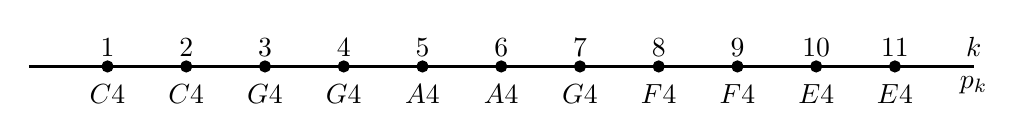
\begin{tikzpicture}
    % Draw number line
    \draw[-, thick] (0,0) -- (12,0) node[below] {$p_k$}  node[above] {$k$};

    % Data
    \foreach \i/\x/\p in {1/C4/1, 2/C4/2, 3/G4/3, 4/G4/4, 5/A4/5, 6/A4/6, 7/G4/7, 8/F4/8, 9/F4/9, 10/E4/10, 11/E4/11} {
      % Draw points and labels
      \filldraw (\i,0) circle (2pt) node[above] {$\p$};
      
      % Draw number scale below the line
      \draw (\i,-0.1) node[below] {$\x$};
    }

  \end{tikzpicture}
  \caption{The first 11 pitches of the 12 variations on Ah vous dirai-je Maman are marked below the 1D axis.}
  \label{subfig:mp}
\end{subfigure}

\vspace{5pt}

\begin{subfigure}{\textwidth}
  \centering
  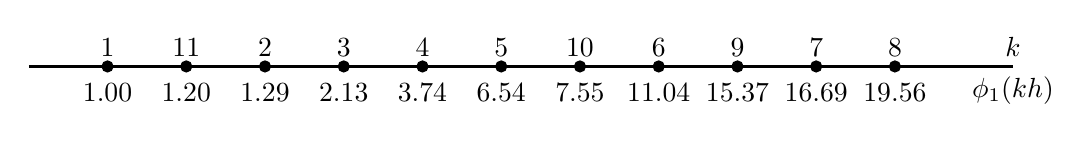
\begin{tikzpicture}
    % Draw number line
    \draw[-, thick] (0,0) -- (12.5,0) node[below] {$\phi_1(kh)$}  node[above] {$k$};

    % Data
    \foreach \i/\x/\p in {1/1.00/1, 2/1.20/11, 3/1.29/2, 4/2.13/3, 5/3.74/4, 6/6.54/5, 7/7.55/10, 8/11.04/6, 9/15.37/9, 10/16.69/7, 11/19.56/8} {
      % Draw points and labels
      \filldraw (\i,0) circle (2pt) node[above] {$\p$};
      
      % Draw number scale below the line
      \draw (\i,-0.1) node[below] {$\x$};
    }

  \end{tikzpicture}
  \caption{The first 11 components from the numerical solution of Lorenz system with initial condition of $(1,1,1)$ are marked below the 1D axis.}
  \label{subfig:traj1}
\end{subfigure}

\vspace{5pt}

\begin{subfigure}{\textwidth}
  \centering
  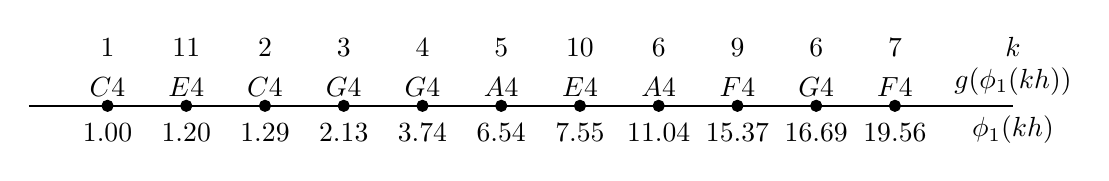
\begin{tikzpicture}
    % Draw number line
    \draw[-, thick] (0,0) -- (12.5,0) node[below] {$\phi_1(kh)$}  node[above] {$g(\phi_1(kh))$} node[above=0.5cm] {$k$};

    % Data
    \foreach \i/\x/\p in {1/1.00/C4, 2/1.20/E4, 3/1.29/C4, 4/2.13/G4, 5/3.74/G4, 6/6.54/A4, 7/7.55/E4, 8/11.04/A4, 9/15.37/F4, 10/16.69/G4, 11/19.56/F4} {
      % Draw points and labels
      \filldraw (\i,0) circle (2pt) node[above] {$\p$};
      
      % Draw number scale below the line
      \draw (\i,-0.1) node[below] {$\x$};
    }
    
    % Display the sequence at each point
    \foreach \i/\x in {1/1, 2/11, 3/2, 4/3, 5/4, 6/5, 7/10, 8/6, 9/9, 10/6, 11/7} {
      \draw (\i,0.5) node[above] {\x};
    }
  \end{tikzpicture}
  \caption{For each component in $\{\phi_1(kh)\}_{k=0}^{10}$, apply the $g(\phi_1(kh))$ mapping.}
  \label{subfig:traj1mp}

\end{subfigure}

\vspace{5pt}

\begin{subfigure}{\textwidth}
  \centering
  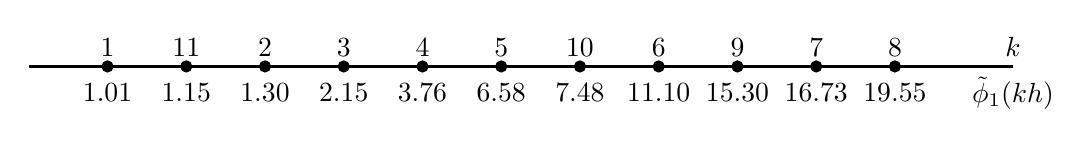
\begin{tikzpicture}
    % Draw number line
    \draw[-, thick] (0,0) -- (12.5,0) node[below] {$\tilde{\phi}_1(kh)$}  node[above] {$k$};

    % Data
    \foreach \i/\x/\p in {1/1.01/1, 2/1.15/11, 3/1.30/2, 4/2.15/3, 5/3.76/4, 6/6.58/5, 7/7.48/10, 8/11.10/6, 9/15.30/9, 10/16.73/7, 11/19.55/8} {
      % Draw points and labels
      \filldraw (\i,0) circle (2pt) node[above] {$\p$};
      
      % Draw number scale below the line
      \draw (\i,-0.1) node[below] {$\x$};
    }

  \end{tikzpicture}
  \caption{The first 11 x-components of the numerical solution of Lorenz system with new initial condition of $(1.01,1,1)$ are marked below the 1D axis.}
  \label{subfig:traj2}

\end{subfigure}

\vspace{5pt}

\begin{subfigure}{\textwidth}
  \centering
  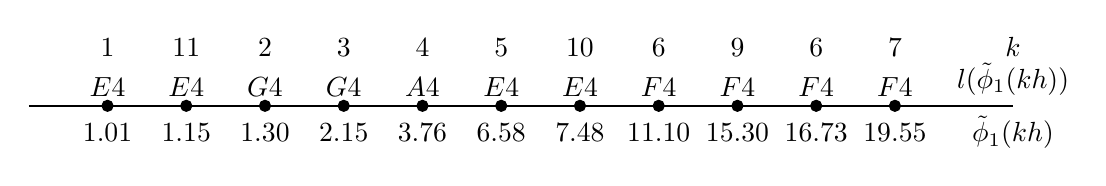
\begin{tikzpicture}
    % Draw number line
    \draw[-, thick] (0,0) -- (12.5,0) node[below] {$\tilde{\phi}_1(kh)$}  node[above] {$l(\tilde{\phi}_1(kh))$} node[above=0.5cm] {$k$};

    % Data
    \foreach \i/\x/\p in {1/1.01/E4, 2/1.15/E4, 3/1.30/G4, 4/2.15/G4, 5/3.76/A4, 6/6.58/E4, 7/7.48/E4, 8/11.10/F4, 9/15.30/F4, 10/16.73/F4, 11/19.55/F4} {
      % Draw points and labels
      \filldraw (\i,0) circle (2pt) node[above] {$\p$};
      
      % Draw number scale below the line
      \draw (\i,-0.1) node[below] {$\x$};
    }
    
    % Display the sequence at each point
    \foreach \i/\x in {1/1, 2/11, 3/2, 4/3, 5/4, 6/5, 7/10, 8/6, 9/9, 10/6, 11/7} {
      \draw (\i,0.5) node[above] {\x};
    }
  \end{tikzpicture}
  \caption{For each component in $\{\tilde{\phi}_1(kh)\}_{k=0}^{10}$, apply the $l(\tilde{\phi}_1(kh))$ mapping.}
  \label{subfig:traj2nmp}

\end{subfigure}

\vspace{5pt}

\begin{subfigure}{\textwidth}
  \centering
  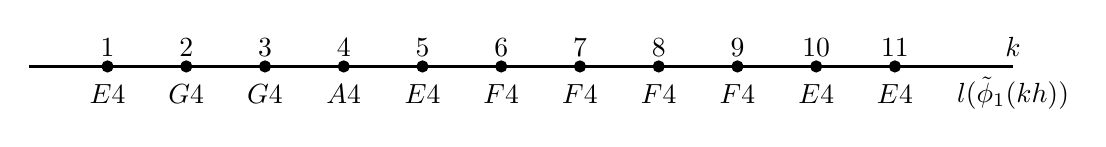
\begin{tikzpicture}
    % Draw number line
    \draw[-, thick] (0,0) -- (12.5,0) node[below] {$l(\tilde{\phi}_1(kh))$}  node[above] {$k$};

    % Data
    \foreach \i/\x/\p in {1/E4/1, 2/G4/2, 3/G4/3, 4/A4/4, 5/E4/5, 6/F4/6, 7/F4/7, 8/F4/8, 9/F4/9, 10/E4/10, 11/E4/11} {
      % Draw points and labels
      \filldraw (\i,0) circle (2pt) node[above] {$\p$};
      
      % Draw number scale below the line
      \draw (\i,-0.1) node[below] {$\x$};
    }

  \end{tikzpicture}
  \caption{The new variation of the first 11 pitches are marked below the 1D axis.}
  \label{subfig:nmp}

\end{subfigure}

\caption{The visualizes how a chaotic mapping method can be used to generate musical variations}
\label{fig:dabby method}
\end{figure}

\subsection{Melodic Variation with Expanded Rhythm Method} 
\label{subsec: melodicvariationwithexpandedrhythm}
For a musical sheet, let $m$ be a positive integer representing a number of notes, $\{p_k\}_{k=0}^{m-1}$be a sequence of music pitches. 
Let $q$ be a positive integer representing a number of expanded notes for each $p_k$, $\{p^\prime_k\}_{k=0}^{mq-1}$ be a sequence of expanded music pitches.

\iffalse
we define a mapping $e$ by $e(p_k) = \{p^\prime_k, p^\prime_{k + 1}, \dots, p^\prime_{k + q} \} $ for all $k \in \{0\}\cup\mathbb{N}_{m-1}$ 
\fi

\begin{example}
\label{ex: MV}
Consider the music piece 12 variations on Ah vous dirai-je Maman in the first bars, illustrated in Figure \ref{fig:MV1}. 
We can convert this musical sheet into a sequence $\{p_k\}_{k=0}^{3}$, where $p_k \in \{ C4, C4, G4, G4 \}$ denotes the musical pitch at index $k$.
Given $q = 4$ be a number of expanded notes for each $p_k$ and $\{p^\prime_k\}_{k=0}^{27}$ be a sequence of expanded music pitches, where $p^\prime_k \in \{ C4, C4, C4, C4, C4, C4, C4, C4, G4, G4, G4, G4, G4, G4, G4, G4 \}$, illustrated in Figure \ref{fig:MV2}.


\iffalse
We can create a mapping $e$ from music pitch to expanded music pitch as follows:
\begin{center}
\begin{tabular}{|c||c|c|c|c|}
\hline
$ p_k $ & C4 & C4 & G4 & G4 \\
\hline
$e(p_k)$ & $\{C4, C4, C4, C4\}$ & $\{C4, C4, C4, C4\}$ & $\{G4, G4, G4, G4\}$ & $\{G4, G4, G4, G4\}$ \\
\hline
$ p_k $ & A4 & A4 & G4 & \\
\hline
$g(p_k)$ & $\{ A4, A4, A4, A4\}$ & $\{ A4, A4, A4, A4\}$ & $\{G4, G4, G4, G4\}$ &   \\
\hline
\end{tabular}
\end{center}
\fi

\end{example}

\begin{figure}
\centering
\includegraphics[trim=1cm 26.5cm 14.325cm 0.02cm, clip, scale=1]{dabby_1.pdf} % trim={left bottom right top}
\caption{The original of 12 variations on Ah vous dirai-je Maman in the first bars.}
\label{fig:MV1} 
\end{figure}

\begin{figure}
\centering
\includegraphics[trim=1cm 26.5cm 8.615cm 0.5cm, clip, scale=0.6]{melody_variation.pdf}
\caption{The melodic variation of Ah vous dirai-je, maman in the first bars.}
\label{fig:MV2}
\end{figure}

\begin{example}
Consider the musical sheet of 12 variations on Ah vous dirai-je Maman in the first 4 bars, illustrated in Figure \ref{fig:DabbyER1}. 
We can convert this musical sheet into a sequence $\{p_k\}_{k=0}^{13}$, where $p_k \in \{C4, C4, G4, G4, A4, A4, G4, F4, F4, E4, E4, D4, D4, C4 \}$ denotes the musical pitch at index $k$. According to example \ref{ex: MV}, $\{p^\prime_k\}_{k=0}^{27}$ be a sequence of expanded music pitches, where $p^\prime_k \in \{ C4, C4, C4, C4, C4, C4, C4, C4, G4, G4, G4, G4, G4, G4, G4, G4 \}$. 
We can apply the procedure of Musical Variations from a Chaotic Mapping to the sequence $\{p^\prime_k\}_{k=0}^{27}$ by using the initial condition $(0.5,0.5,0.5)$ and new trajectory initial condition $(0.6,0.5,0.5)$. Which produce a new sequence $\{l(\tilde{\phi}_1(kh))\}_{k = 0}^{15}$, where $l(\tilde{\phi}_1(kh)) \in \{C4, G4, D4, A4, A4, E4, F4, F4, F4, F4, E4, G4, D4, \\ C4, C4, C4 \} $. 
This new sequence can be converted to musical notation, as shown in Figure \ref{fig:DabbyER2}.
Since this method uses the new note duration to create a new variation (visualized in Figure \ref{fig2:dabbymv method}), the resulting changes in the sequence compared to the original sequence are different. The notes in the new sequence are more numerous compared to the original sequence which have only 4 notes.
\end{example}

\begin{figure}
\centering
\includegraphics[trim=1cm 26.5cm 8.07cm 0.02cm, clip, scale=1]{dabby_1.pdf} % trim={left bottom right top}
\caption{The original of 12 variations on Ah vous dirai-je Maman in the first 4 bars.}
\label{fig:DabbyER1} 
\end{figure}

\begin{figure}
\centering
\includegraphics[trim=1cm 26.5cm 8.65cm 0.5cm, clip, scale=1]{dabby_melody_variation.pdf}
\caption{The new variation with melodic variation of Ah vous dirai-je, maman in the first bars, generated by the Initial Condition $(0.6, 0.5, 0.5)$.} 
\label{fig:DabbyER2}
\end{figure}

\begin{figure}
\centering

\begin{subfigure}{\textwidth}
  \centering
  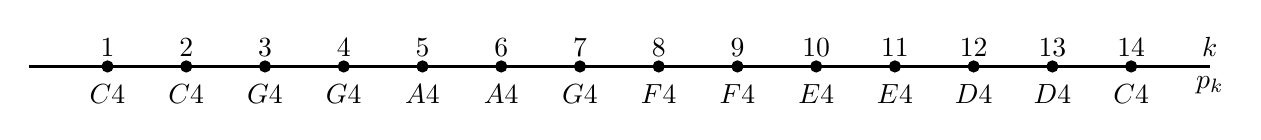
\begin{tikzpicture}
    % Draw number line
    \draw[-, thick] (0,0) -- (15,0) node[below] {$p_k$}  node[above] {$k$};

    % Data
    \foreach \i/\x/\p in {1/C4/1, 2/C4/2, 3/G4/3, 4/G4/4, 5/A4/5, 6/A4/6, 7/G4/7, 8/F4/8, 9/F4/9, 10/E4/10, 11/E4/11, 12/D4/12, 13/D4/13, 14/C4/14} {
      % Draw points and labels
      \filldraw (\i,0) circle (2pt) node[above] {$\p$};
      
      % Draw number scale below the line
      \draw (\i,-0.1) node[below] {$\x$};
    }

  \end{tikzpicture}
  \caption{The first 14 pitches of the 12 variations on Ah vous dirai-je Maman are marked below the 1D axis.}
  \label{subfig2:mp}
\end{subfigure}

\vspace{5pt}

\begin{subfigure}{\textwidth}
  \centering
  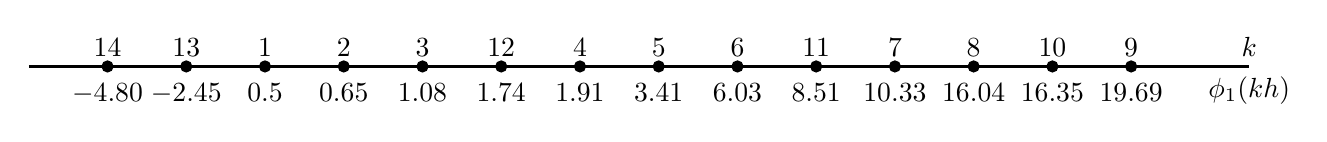
\begin{tikzpicture}
    % Draw number line
    \draw[-, thick] (0,0) -- (15.5,0) node[below] {$\phi_1(kh)$}  node[above] {$k$};

    % Data
    \foreach \i/\x/\p in {1/-4.80/14, 2/-2.45/13, 3/0.5/1, 4/0.65/2, 5/1.08/3, 6/1.74/12, 7/1.91/4, 8/3.41/5, 9/6.03/6, 10/8.51/11, 11/10.33/7, 12/16.04/8, 13/16.35/10, 14/19.69/9} {
      % Draw points and labels
      \filldraw (\i,0) circle (2pt) node[above] {$\p$};
      
      % Draw number scale below the line
      \draw (\i,-0.1) node[below] {$\x$};
    }

  \end{tikzpicture}
  \caption{The first 14 components from the numerical solution of Lorenz system with initial condition of $(0.5,0.5,0.5)$ are marked below the 1D axis.}
  \label{subfig2:traj1}
\end{subfigure}

\vspace{5pt}

\begin{subfigure}{\textwidth}
  \centering
  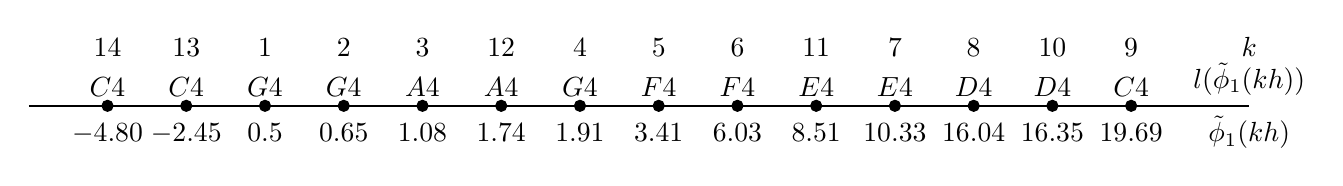
\begin{tikzpicture}
    % Draw number line
    \draw[-, thick] (0,0) -- (15.5,0) node[below] {$\tilde{\phi}_1(kh)$}  node[above] {$l(\tilde{\phi}_1(kh))$} node[above=0.5cm] {$k$};

    % Data
    \foreach \i/\x/\p in {1/-4.80/C4, 2/-2.45/C4, 3/0.5/G4, 4/0.65/G4, 5/1.08/A4, 6/1.74/A4, 7/1.91/G4, 8/3.41/F4, 9/6.03/F4, 10/8.51/E4, 11/10.33/E4, 12/16.04/D4, 13/16.35/D4, 14/19.69/C4} {
      % Draw points and labels
      \filldraw (\i,0) circle (2pt) node[above] {$\p$};
      
      % Draw number scale below the line
      \draw (\i,-0.1) node[below] {$\x$};
    }
    
    % Display the sequence at each point
    \foreach \i/\x in {1/14, 2/13, 3/1, 4/2, 5/3, 6/12, 7/4, 8/5, 9/6, 10/11, 11/7, 12/8, 13/10, 14/9} {
      \draw (\i,0.5) node[above] {\x};
    }
  \end{tikzpicture}
  \caption{For each component in $\{\phi_1(kh)\}_{k=0}^{13}$, apply the $g(\phi_1(kh))$ mapping.}
  \label{subfig2:traj1mp}

\end{subfigure}

\vspace{5pt}

\begin{subfigure}{\textwidth}
  \centering
  \small{
  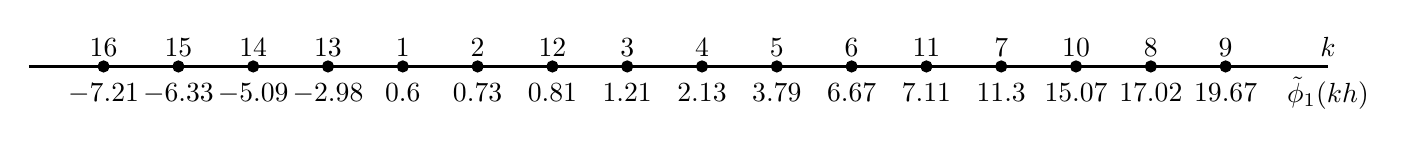
\begin{tikzpicture}
    % Draw number line
    \draw[-, thick] (0,0) -- (16.5,0) node[below] {$\tilde{\phi}_1(kh)$}  node[above] {$k$};

    % Data
    \foreach \i/\x/\p in {1/-7.21/16, 2/-6.33/15, 3/-5.09/14, 4/-2.98/13, 5/0.6/1, 6/0.73/2, 7/0.81/12, 8/1.21/3, 9/2.13/4, 10/3.79/5, 11/6.67/6, 12/7.11/11, 13/11.3/7, 14/15.07/10, 15/17.02/8, 16/19.67/9} {
      % Draw points and labels
      \filldraw (\i*0.95,0) circle (2pt) node[above] {$\p$};
      
      % Draw number scale below the line
      \draw (\i*0.95,-0.1) node[below] {$\x$};
    }

  \end{tikzpicture}}
  \caption{The first 16 x-components of the numerical solution of Lorenz system with new initial condition of $(0.6,0.5,0.5)$ are marked below the 1D axis.}
  \label{subfig2:traj2}

\end{subfigure}

\vspace{5pt}

\begin{subfigure}{\textwidth}
  \centering
  \small{
  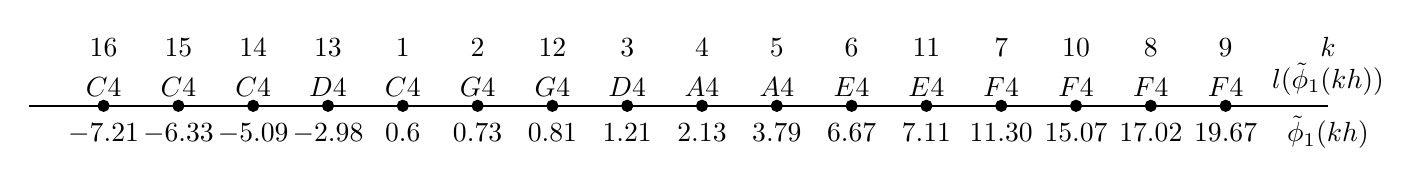
\begin{tikzpicture}
    % Draw number line
    \draw[-, thick] (0,0) -- (16.5,0) node[below] {$\tilde{\phi}_1(kh)$}  node[above] {$l(\tilde{\phi}_1(kh))$} node[above=0.5cm] {$k$};

    % Data
    \foreach \i/\x/\p in {1/-7.21/C4, 2/-6.33/C4, 3/-5.09/C4, 4/-2.98/D4, 5/0.6/C4, 6/0.73/G4, 7/0.81/G4, 8/1.21/D4, 9/2.13/A4, 10/3.79/A4, 11/6.67/E4, 12/7.11/E4, 13/11.30/F4, 14/15.07/F4, 15/17.02/F4, 16/19.67/F4} {
      % Draw points and labels
      \filldraw (\i*0.95,0) circle (2pt) node[above] {$\p$};
      
      % Draw number scale below the line
      \draw (\i*0.95,-0.1) node[below] {$\x$};
    }
    
    % Display the sequence at each point
    \foreach \i/\x in {1/16, 2/15, 3/14, 4/13, 5/1, 6/2, 7/12, 8/3, 9/4, 10/5, 11/6, 12/11, 13/7, 14/10, 15/8, 16/9} {
      \draw (\i*0.95,0.5) node[above] {\x};
    }
  \end{tikzpicture}}
  \caption{For each component in $\{\tilde{\phi}_1(kh)\}_{k=0}^{15}$, apply the $l(\tilde{\phi}_1(kh))$ mapping.}
  \label{subfig2:traj2nmp}

\end{subfigure}

\vspace{5pt}

\begin{subfigure}{\textwidth}
  \centering
  \small{
  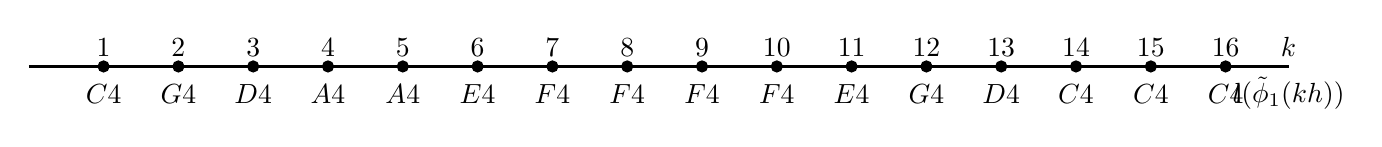
\begin{tikzpicture}
    % Draw number line
    \draw[-, thick] (0,0) -- (16,0) node[below] {$l(\tilde{\phi}_1(kh))$}  node[above] {$k$};

    % Data
    \foreach \i/\x/\p in {1/C4/1, 2/G4/2, 3/D4/3, 4/A4/4, 5/A4/5, 6/E4/6, 7/F4/7, 8/F4/8, 9/F4/9, 10/F4/10, 11/E4/11, 12/G4/12, 13/D4/13, 14/C4/14, 15/C4/15, 16/C4/16} {
      % Draw points and labels
      \filldraw (\i*0.95,0) circle (2pt) node[above] {$\p$};
      
      % Draw number scale below the line
      \draw (\i*0.95,-0.1) node[below] {$\x$};
    }

  \end{tikzpicture}}
  \caption{The new variation of the first 16 pitches are marked below the 1D axis.}
  \label{subfig2:nmp}

\end{subfigure}

\caption{The visualizes how a chaotic mapping with melodic variation method can be used to generate musical variations}
\label{fig2:dabbymv method}
\end{figure}

\section{Discussion}
\label{sec: discussion}
This section explores the potential of Combination of Musical Variations from a Chaotic Mapping and Melodic Variation with Expanded Rhythm technique for generating musical variations. It analyzes the impact of this approach on the resulting variations compared to traditional melodic variation techniques. 

\subsection{Strengths of the Combined Approach}

The combined approach shows potential in generating interesting musical variations, as shown in the new variations with melodic variation of Pachelbel's Canon \cite{pachelbel_canon_2005} (Figure \ref{fig:NCND}) compared to the original melody (Figure \ref{fig:OCND}).

This method appears to be particularly effective for pieces with a larger range of musical pitches, as exemplified by Pachelbel's Canon. The additional pitches provide more material for the chaotic mapping and melodic variation techniques to manipulate, leading to richer and more diverse variations.

\begin{figure}
\centering
\includegraphics[trim=1cm 26.5cm 1cm 0.5cm, clip, scale=0.6]{Original_CND.pdf}
\caption{The original of Pachelbel's Canon in the first 10 bars.} 
\label{fig:OCND}
\end{figure}

\begin{figure}
\centering
\includegraphics[trim=1cm 20.3cm 1cm 0.5cm, clip, scale=0.6]{New_CND.pdf}
\caption{The new variation with melodic variation of Pachelbel's Canon in the first 10 bars (including 2 additional bars at the end of the 10th bar).} 
\label{fig:NCND}
\end{figure}

\subsection{Weaknesses of the Combined Approach}

Let's consider the musical sheet for Vanessa Carlton's A Thousand Miles (Figure \ref{fig:OATM}) and the new variation with melodic variation (Figure \ref{fig:NATM}). This result shows that using musical sheets with too many musical note durations can lead to new variations with melodies that are difficult to play and listen to. This is a major weakness of this method.

\begin{figure}
\centering
\includegraphics[trim=1cm 26.5cm 1cm 0.5cm, clip, scale=0.6]{Original_ATM.pdf}
\caption{The original of Vanessa Carlton - A Thousand Miles in the first 3 bars.} 
\label{fig:OATM}
\end{figure}

\begin{figure}
\centering
\includegraphics[trim=1cm 23.75cm 1cm 0.5cm, clip, scale=0.6]{New_ATM.pdf}
\caption{The new variation with melodic variation of Vanessa Carlton - A Thousand Miles in the first 3 bars.} 
\label{fig:NATM}
\end{figure}

\subsection{Limitations and Considerations}

Further evaluation with a wider range of musical pieces is necessary to determine the generalizability of these observations. The effectiveness of the combined approach might vary depending on the musical style and characteristics of the original piece.

The computational complexity of the chaotic mapping technique should also be considered. While it offers a powerful approach for variation, it might require more processing power compared to simpler melodic variation methods.

\subsection{Future Directions}

Exploring different parameters and configurations within the chaotic mapping and melodic variation techniques could potentially lead to a wider range of variation styles and outcomes.

Investigating methods for user control over the variation process would be valuable. This could allow musicians to tailor the generated variations to their specific creative goals.

Integrating this combined approach into music composition tools could provide composers with a valuable tool for generating new musical ideas and exploring creative possibilities.

\section{Conclusion}
\label{sec: conclusion}
The proposed method, leveraging the power of chaotic systems, offers a promising approach to music composition, addressing the limitations of existing AI techniques and providing composers with a tool to generate novel, unpredictable, and diverse musical compositions while reducing computational resource demands. This method has the potential to stimulate creativity, alleviate composer's burnout, and expand the boundaries of musical expression, paving the way for a new era of music creation driven by chaos and innovation.

\iffalse
\begin{figure}
\centering
\begin{subfigure}{0.45\textwidth}
  \centering
  \includegraphics[scale=0.55]{Dabby_process.pdf}
  \caption{Flowchart of musical variations from a chaotic mapping (Diana S. Dabby)}
\end{subfigure}
\begin{subfigure}{0.45\textwidth}
  \centering
  \includegraphics[scale=0.55]{Real_process.pdf}
  \caption{Flowchart of combining musical variations from a chaotic mapping (Diana S. Dabby) and melodic variation with expanded rhythm}
\end{subfigure}
\caption{Flowcharts of musical variations}
\label{fig:combined_flowcharts}
\end{figure}
\fi

\printbibliography

\end{document}